\documentclass[11pt, oneside]{article} 
\usepackage{geometry}
\geometry{letterpaper} 
\usepackage{graphicx}
	
\usepackage{amssymb}
\usepackage{amsmath}
\usepackage{parskip}
\usepackage{color}
\usepackage{hyperref}

\graphicspath{{/Users/telliott_admin/Tex/png/}}
% \begin{center} 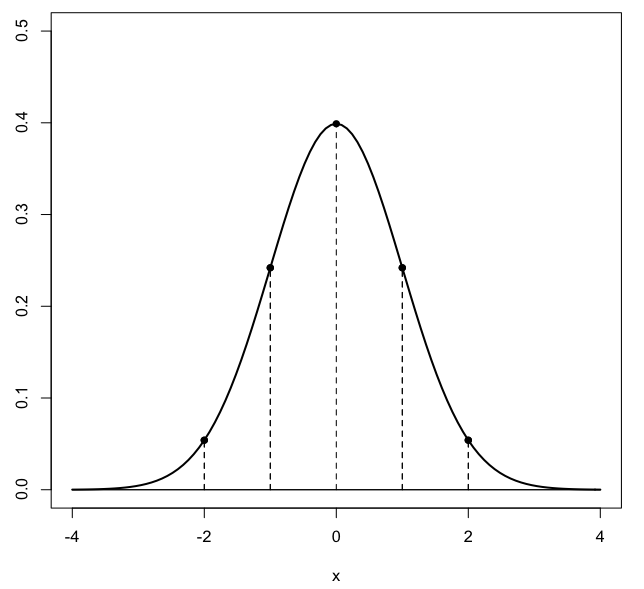
\includegraphics [scale=0.4] {gauss3.png} \end{center}

\title{Introduction to the exponential}
\date{}

\begin{document}
\maketitle
\Large

\subsection*{Principal and interest}
Suppose I put $100$ dollars in the bank, and the people at the bank say that after one year, they will give me an additional $\$10$ at that time.  We say that they are paying $10\%$ interest for the year on the principal $P$ of $\$100$.

However, suppose I bargain with them.  I get them to promise to pay me half the interest ($5\%$) at the six-month mark, and the rest after one year.  My account will hold $\$105$ after six months, and the interest due for the second half will be $5\%$ of $\$105$, which is $\$5.25$ for a total of $\$10.25$.

The equation to describe this situation is that if the rate of interest for the year is $r$ and the year is broken up into $n$ periods when interest will be paid, the total amount at the end will be:
\[ A = P(1 + \frac{r}{n})^n \]

In the example, we have $r = 0.10$ and $n = 2$ so
\[ A = 100 (1 + 0.05)^{2} = 110.25 \]

This is compound interest.  If there are additional years $t$, the exponent will be $nt$ rather than $n$.

And now we start wondering what happens if the bank pays every month so that $n=12$ or every day so $n=365$ or even every second.  What happens if the interest is compounded \emph{continuously}?
\[ A = \lim_{n \rightarrow \infty} P \ [ \ (1 + \frac{r}{n})^{n} \ ] \]

Now it turns out that in the limit as $n$ approaches $\infty$ these two expressions are equal
\[ (1 + \frac{r}{n})^n = \ [ \ (1 + \frac{1}{n})^n \ ]^r \]
The same factor $r$ can be either in the numerator of the second term inside or up in the exponent outside.  

A quick proof is:
\[ \lim_{n \rightarrow \infty} (1 + \frac{r}{n})^{n}  \]
\[ = \lim_{n \rightarrow \infty} (1 + \frac{r}{n})^{(n/r)r} \]
Define $m = n/r$ and so as $n \rightarrow \infty$, so does $m \rightarrow \infty$ and then we have
\[ \lim_{m \rightarrow \infty} (1 + \frac{1}{m})^{(m)r} \]
and the $r$ is outside.  $m$ is just a dummy variable so we write:
\[ \lim_{n \rightarrow \infty} \ [ \  (1 + \frac{1}{n})^{n} \ ]^r \]

Therefore, going back to what we were working on, let us bring out the factor $r$ and obtain
\[ A = P(1 + \frac{1}{n})^{nr} \]
\[ A = P \ [ \ (1 + \frac{1}{n})^{n} \ ] ^r \]

Thus, the important question is, what is the value of this expression?
\[ A = \lim_{n \rightarrow \infty} (1 + \frac{1}{n})^{n} \]

It does not depend on $r$.  It will turn out that this limit is equal to the number $e$.
\[ e = 2.71828\ 18284\ 59045 \dots \]

First, though, let us review some properties of logarithms.

\subsection*{working with logarithms}

The logarithm and exponential functions are inverses.  If we have that
\[ y = b^x \]
for some $b > 0, b \ne 1$, then we say that
\[ x = \log_b \ y \]
Putting them together
\[ y = b^{\ \log_b y} \]
The usual bases are $10$ (common logarithm, $\log_{10}$, or just $\log$), $e$ (natural logarithm or $\ln$), and $2$ (binary logarithm or $\log_2$).

The rules for exponents are simple, if $p$ and $q$ are two numbers and we know the logarithms of $p$ and $q$ to base $b$
\[ p = b^{u}; \ \ \ q = b^{v} \]
then their product can be computed as:
\[ pq = b^{u} \cdot b^{v} = b^{u + v} \]
It helps if we can actually compute $b^{u+v}$.  In the old days there were tables of logarithms, so you just looked up the answer in the table.

The second rule is that:
\[ (b^u)^v = b^{uv} \] 
And in terms of logarithms we write
\[ \log_b (b^u)^v = \log b^{uv} = v \log_b (b^u) \]

For example 
\[ 2^2 = 2 \times 2 = 4 \] 
\[ 2^3 = 2 \times 2 \times 2 = 8 \]
\[ 4 \times 8 = 2^2 \times 2^3 = 2^{2 + 3} = 2^5 \]
\[ = 2 \times  2 \times 2 \times 2 \times 2 = 32 \]
and
\[ (2^2)^3 = 4^3 = 64 = 2^6 = 2^{2 \times 3} \]

Here is a plot of $\log_{10}(x)$ and $\ln x$:
\begin{center} 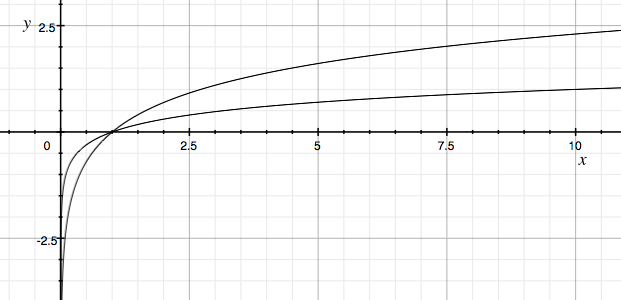
\includegraphics [scale=0.5] {log1.png} \end{center}
The first function reaches the value $1$ when $x=10$ and the second reaches the value $1$ when $x=e$.  Both have the value $0$ at $x=1$ because $b^0 = 1$ for any base, so the logarithm to any base of $1$ is equal to $0$.

It turns out that if we take the logarithm of $x$ (where $x$ is any number $> 1$) to two \emph{different} bases, the ratio of the logarithms is a constant, independent of the value of $x$.  

\subsection*{change of bases}

This is nicely shown by the change of bases formula.
\[ \log_b x = \frac{\log_a x}{\log_a b} \]

Start with an expression with $b$ as the base:
\[ y = b^x \]
and by the definition of the logarithm
\[ x = \log_b y \]

To derive the formula, take the logarithm to the base $a$ on both sides of the first expression:
\[ \log_a y = \log_a (b^x) \]

Now, just invoke the second rule on the right-hand side
\[ = x \log_a b \]
and substitute for $x$ from the second expression above
\[ = \log_b y \log_a b \]
We're basically done.

$y$ can be any value, so replace it by $x$
\[ \log_a x = \log_b x \log_a b \]
Rearranging:
\[ \log_b x = \frac{\log_a x}{\log_a b} \]

One way I remember this is that first the logarithms to different bases are connected by some constant $k$
\[ \log_b x = k \log_a x \]
and we substitute for $k$ the inverse of the log to the \emph{same} base as we have in the numerator:
\[ \log_b x = \frac{\log_a x}{\log_a b} \]
that is, I remember that we want $\log_a$ something \emph{over }$\log_a$ something on the right. 

Alternatively, you might look at the other formula
\[ \log_a x = \log_a b \log_b x  \]
and imagine the $b$'s canceling in some way.

One other thing we can do is to set $x=a$ in the above formula.  We start from
\[ \log_b x = \frac{\log_a x}{\log_a b} \]
then with $x=a$
\[ \log_b a = \frac{\log_a a}{\log_a b} \]
but $\log_a a = 1$ so
\[ \log_b a = \frac{1}{\log_a b} \]

And that makes perfect sense.  If we multiply by some factor $k$ to convert from the logarithm in base $a$ to base $b$, we must multiply by the inverse of the same factor to convert back again.

For the figure above of the common log (base 10) and the natural logarithm, $\ln 10 = 2.303$, and that looks about right, when $x=10$ the first function is $1.0$ and the second one is about $2.3$.

The logarithm and the exponential are inverse functions, we can see that if we plot them together:
\begin{center} 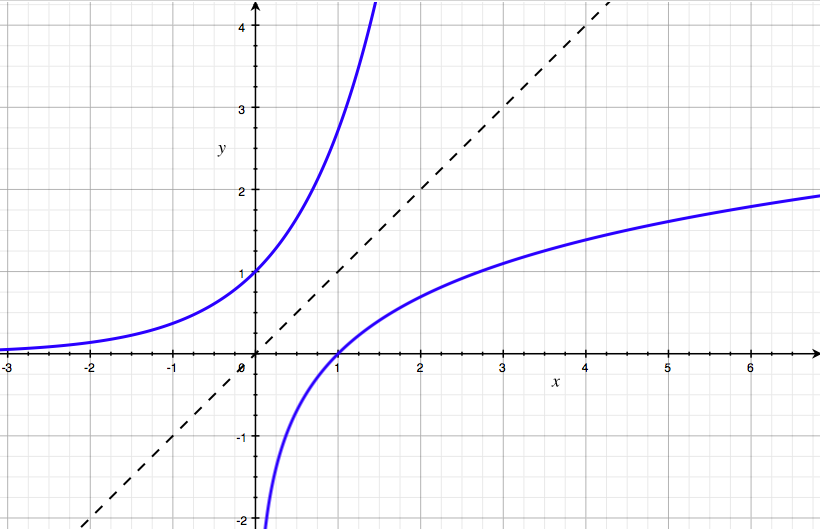
\includegraphics [scale=0.5] {log2.png} \end{center}
The upper curve is $y = e^x$ and the lower one is $y = \ln x$.
As inverse functions, they are symmetric about the line $y=x$.  

\subsection*{fractional exponents}
The introduction above dealt mainly with integer exponents, but of course you know that the practical use of logarithms depends on fractional values.  The simplest way to see how this works is to consider the square root.
\[ \sqrt{2} \times \sqrt{2} = 2 \]
If we think about what the exponent $u$ to the base $2$ would be such that
\[ 2^u = \sqrt{2} \]
We observe that by the rules for exponents
\[ \sqrt{2} \times \sqrt{2} = 2^u \times 2^u = 2^{u+u} = 2^1 \]
That is
\[ u + u = 1 \]
so $u = 1/2$.  By the same logic the $n^{\text{th}}$ root of $b$ is $b^{1/n}$.  And of course 
\[ (b^2)^{1/2} = b^{2 \times 1/2} = b^1 \]
Feynman has a nice description of how logarithms were calculated (see Lectures, volume 1, Chapter 22, Algebra;  

\url{http://www.feynmanlectures.caltech.edu/I_22.html})

The basic idea is to take repeated square roots of the base ($10$), and then combine those to form the required value.

\subsection*{Less than 1}
Fractional exponents leads to consideration of $0 < x < 1$.  Write
\[ x \ \frac{1}{x} = 1 \]
Take the logarithm of both sides
\[ \log(x \ \frac{1}{x} ) = \log 1 = 0 \]
\[ = \log x + \log \frac{1}{x} \]
Thus
\[ \log \frac{1}{x} = - \log x \]

\end{document}  